\chapter{TỔNG QUAN}
    \section{Tìm hiểu về AGVs}
    \subsection{Tổng quan về AGVs}
    \hspace*{0.6cm}AGVs (Automated Guided Vehicles) hay còn gọi là hệ thống robot tự hành, là các robot có khả năng tự lái, sử dụng động cơ điện,
    tích hợp điều khiển trong một phần mềm hệ điều hành chính để có khả năng lập trình lựa chọn đường đi, điểm đến và tránh va chạm, 
    có nhiệm vụ chuyên chở, xếp dỡ hàng hóa, vật liệu trong các nhà máy, kho xưởng, v.v.
    
    \section{Sơ lược về robot dò line}
        \hspace*{0.6cm}Robot dò line (Line following Robot) là một dạng robot di động (mobile robot) di
        chuyển bằng bánh xe. Robot sẽ di chuyển bám theo các đường line được kẻ/vẽ/dán trên
        mặt đất. Quỹ đạo di chuyển của robot phụ thuộc vào sa bản của hệ thống các đường line
        được kẻ/vẽ/dán sẵn. Một robot dò line gồm các yếu tố: sơ đồ nguyên lý, loại cảm biến,
        động cơ, cấu trúc điều khiển. \\
        \hspace*{0.6cm}Hiện nay, có rất nhiều kết cấu cơ khí được thiết kế để cải thiện khả năng di chuyển
        của robot dò line như đáp ứng tốc độ, độ chính xác bám line,\dots. Các kết cấu hiện nay
        phổ biến là: cấu trúc hai bánh, ba bánh, bốn bánh, bánh xích, \dots \\
        \hspace*{0.6cm} Trong phạm vi của đề tài, nhóm hướng đến thiết kế robot dò line bám đường và
        có khả năng nhận diện được màu sắc của kiện hàng được đặt lên xe tại khu vực tải hàng, từ đó phân phối hàng hóa đến vị trí kết thúc theo quỹ đạo có màu sắc tương ứng với màu sắc của gói hàng.\\
        \hspace*{0.6cm}Trong phạm vi đề tài, nhóm hướng đến thiết kế 1 AGV bám line có khả năng vận chuyển tải hàng có khối lượng 1kg đặt trong hộp đựng kích thước 85 x 55 x 72 mm.


    \section{Các sản phẩm ở trong và ngoài nước}
    \hspace*{0.6cm}Vì hướng đến thiết kế một AGV vừa có khả năng bám đường line và vừa có khả năng tải hàng, nhóm tiến hành vừa tham khảo nguyên lý cơ khí và cảm biến của những loại xe bám line và AGV tải hàng. 
    \subsection{Robot Zumo Slim}
        \hspace*{0.6cm}Robot Zumo Slim là robot của anh Zeremy trong cuộc thi LVBots line following.
        \begin{itemize}
            \item Sơ đồ nguyên lý cơ khí:
            \begin{figure}[H]
                \begin{subfigure}{0.5\textwidth}
                \centering
                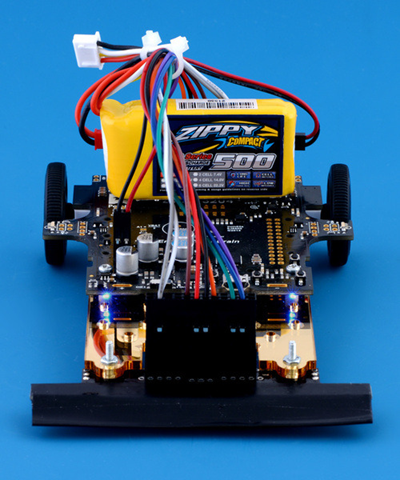
\includegraphics[width=0.5\linewidth, right]{pictures/chapter1/chapter1_pic_10a_zumo_slim.png} 
                \label{chap1_pic10a}
                \end{subfigure}
                \begin{subfigure}{0.6\textwidth}
                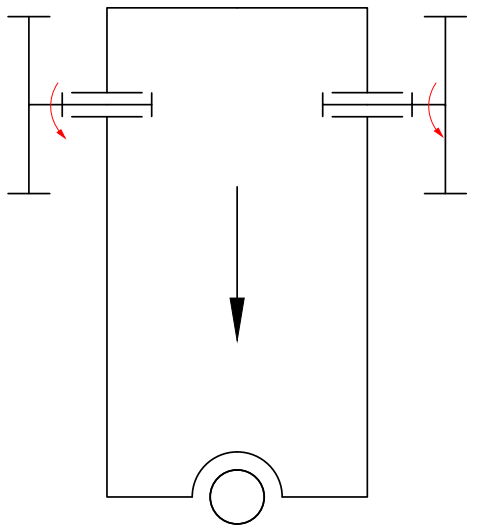
\includegraphics[width=0.5\linewidth]{pictures/chapter1/chapter1_pic_10b_zumo_slim.png}
                \label{chap1_pic10b}
                \end{subfigure}
                \caption{Robot Zumo Slim}
                \label{chap1_pic10}
            \end{figure}
            % image 10
            \item Các thành phần của robot:
                \begin{itemize}[label=\textendash]
                    \item Động cơ DC có encoder, có hộp số tỉ lệ 10:1.
                    \item Cảm biến: Cảm biến line và cảm biến tiệm cận được gắn ở đầu xe.
                    \item Vi điều khiển: Zumo's ATmega32U4.
                    \item Bánh xe: Sử dụng 3 bánh, 2 bánh chủ động phía sau và 1 bánh bị động tự lựa phía trước.
                \end{itemize}
        \end{itemize}

    \subsection{Robot CompaRob}
        \hspace*{0.6cm} CompaRob là 1 dạng robot vận chuyển xe đẩy mua hàng, có khả năng vận chuyển hàng hóa.
        \begin{itemize}
            \item Sơ đồ nguyên lý cơ khí:
            \begin{figure}[H]
                \begin{subfigure}{0.5\textwidth}
                \centering
                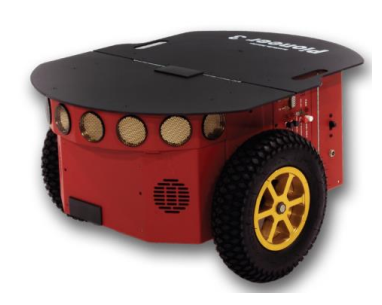
\includegraphics[width=0.6\linewidth, right]{pictures/chapter1/chapter1_pic11a_comparob.png} 
                \label{chap1_pic11a}
                \end{subfigure}
                \begin{subfigure}{0.6\textwidth}
                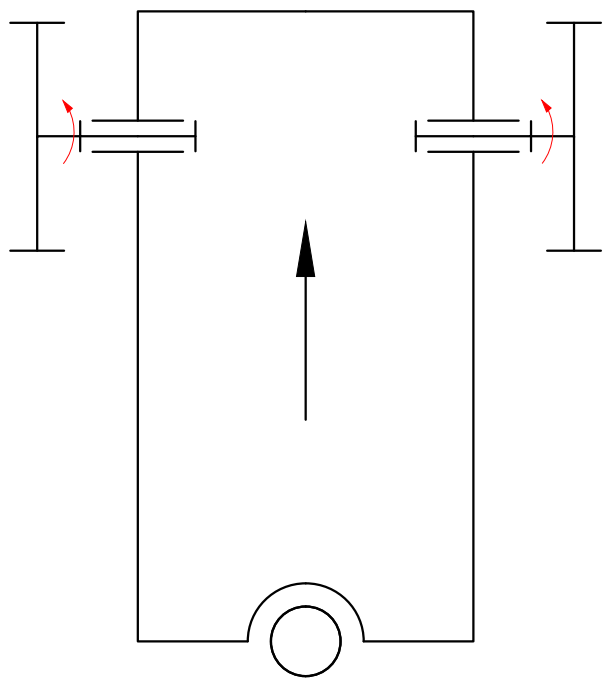
\includegraphics[width=0.5\linewidth]{pictures/chapter1/chapter1_pic11b_pinto.png}
                \label{chap1_pic11b}
                \end{subfigure}
                \caption{Robot Pinto}
                \label{chap1_pic11}
            \end{figure}
            %image 11
            \item Các thông số kĩ thuật của robot:
                \begin{itemize}[label=\textendash]
                    \item Kích thước $455 \times 381 \times 237 \,\mathrm{mm}$, trọng lượng 9 kg, thời lượng pin 9h.
                    \item Tốc độ tối đa $1.2 \,\mathrm{m/s}$.
                    \item Đường kính bánh chủ động $534 \,\mathrm{mm}$.
                    \item Bánh xe: Sử dụng 3 bánh, 2 bánh chủ động phía trước và 1 bánh bị động tự lựa phía sau.
                \end{itemize}
        \end{itemize}



    \subsection{AGV Weasel (Low structure)}
        \hspace*{0.6cm} AGV Weasel của hãng Schaefer chuyên dùng để vận chuyển hàng hóa trong nhà kho hoặc trong các nhà máy sản xuất tự động.
        \begin{itemize}
            \item Sơ đồ nguyên lý cơ khí:
            \begin{figure}[H]
                \begin{subfigure}{0.5\textwidth}
                \centering
                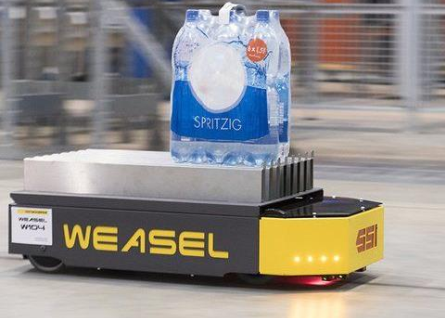
\includegraphics[width=0.6\linewidth, right]{pictures/chapter1/chapter1_pic12a_weasle.png} 
                \label{chap1_pic12a}
                \end{subfigure}
                \begin{subfigure}{0.7\textwidth}
                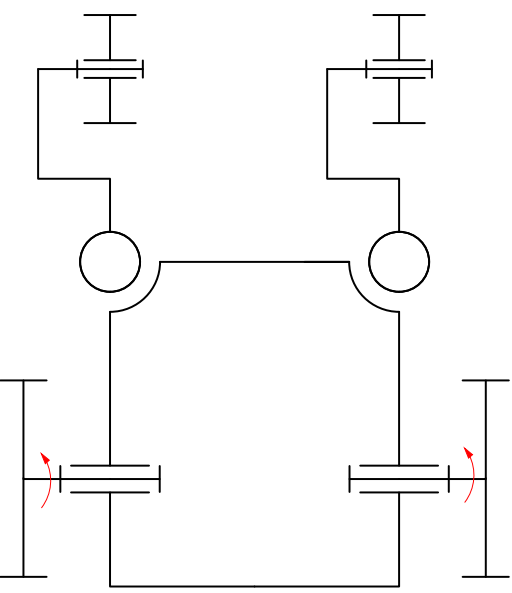
\includegraphics[width=0.55\linewidth]{pictures/chapter1/chapter1_pic12b_newbie.png}
                \label{chap1_pic12b}
                \end{subfigure}
                \caption{Robot Newbie}
                \label{chap1_pic12}
            \end{figure}
            %image 12
            \item Các thông số kĩ thuật của robot:
                \begin{itemize}[label=\textendash]
                    \item Kích thước $600 \times 400 \times 510 \,\mathrm{mm}$, trọng lượng 35 kg, thời lượng pin 16h.
                    \item Tốc độ tối đa $1 \,\mathrm{m/s}$.
                    \item Đường kính bánh chủ động $150 \,\mathrm{mm}$.
                    \item Bánh xe: Sử dụng 4 bánh, 2 bánh chủ động phía sau và 2 bánh bị động tự lựa phía trước.
                \end{itemize}
        \end{itemize}



    \subsection{Robot Fireball}
        \hspace*{0.6cm}Robot Fireball tham gia kì thi ChiBots ở Mỹ mùa hè năm 2010.
        \begin{itemize}
            \item Sơ đồ nguyên lý cơ khí:
            \begin{figure}[H]
                \begin{subfigure}{0.5\textwidth}
                \centering
                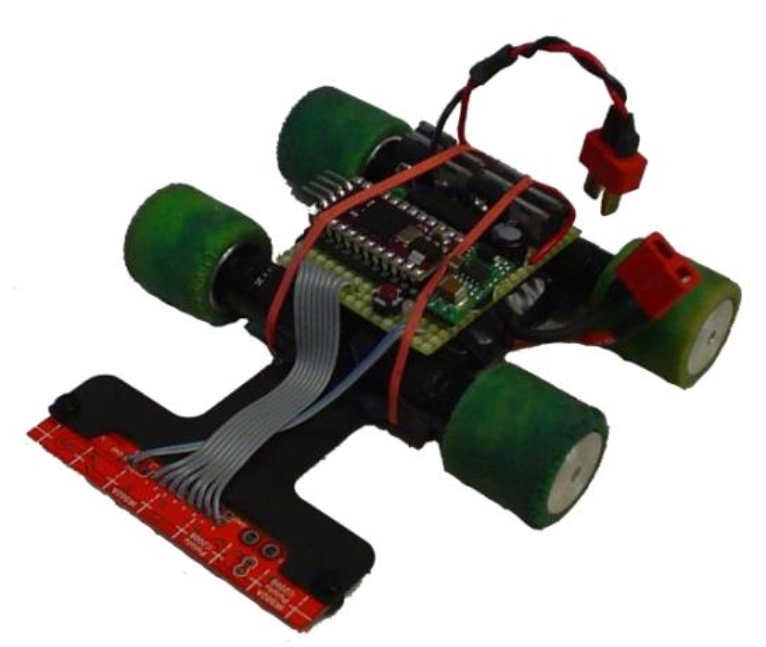
\includegraphics[width=0.6\linewidth, right]{pictures/chapter1/chapter1_pic13a_fireball.png} 
                \label{chap1_pic13a}
                \end{subfigure}
                \begin{subfigure}{0.6\textwidth}
                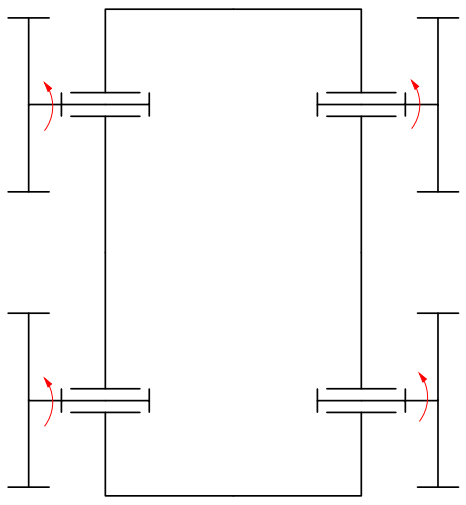
\includegraphics[width=0.5\linewidth]{pictures/chapter1/chapter1_pic13b_fireball.png}
                \label{chap1_pic13b}
                \end{subfigure}
                \caption{Robot Fireball}
                \label{chap1_pic13}
            \end{figure}
            %image 13
            \item Các thành phần của robot:
                \begin{itemize}[label=\textendash]
                    \item Động cơ: 4 động cơ DC có Encoder, sử dụng driver SN754410.
                    \item Cảm biến: Dùng bộ cảm biến 8 hồng ngoại Pololu QTR-8RC, được đặt thành dãy ở đầu xe.
                    \item Bánh xe: Sử dụng 4 bánh đều là bánh chủ động.
                \end{itemize}
        \end{itemize}



    \subsection{Robot Khepera IV}
        \hspace*{0.6cm}Robot Khepera IV là robot dạng tròn, dẫn động vi sai.
        \begin{itemize}
            \item Sơ đồ nguyên lý cơ khí:
            \begin{figure}[H]
                \begin{subfigure}{0.5\textwidth}
                \centering
                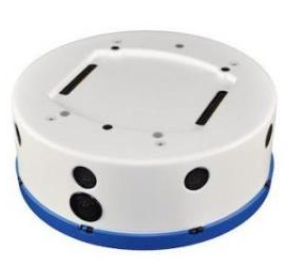
\includegraphics[width=0.6\linewidth, right]{pictures/chapter1/chapter1_pic14a_kheperaIV.png} 
                \label{chap1_pic14a}
                \end{subfigure}
                \begin{subfigure}{0.6\textwidth}
                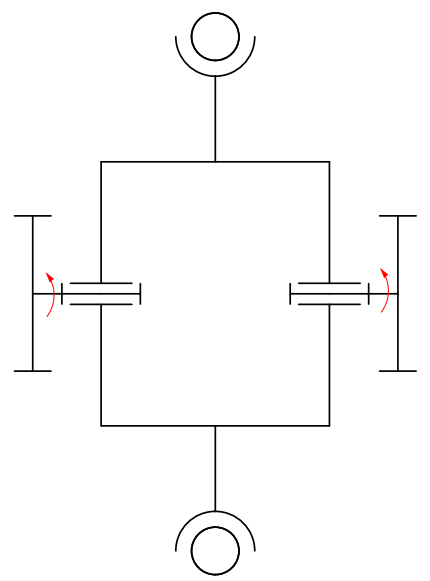
\includegraphics[width=0.5\linewidth]{pictures/chapter1/chapter1_pic14b_kheperaIV.png}
                \label{chap1_pic14b}
                \end{subfigure}
                \caption{Robot Khepera IV}
                \label{chap1_pic14}
            \end{figure}
            %image 14
            \item Các thành phần của robot:
                \begin{itemize}[label=\textendash]
                    \item Cảm biến: Dùng bộ cảm biến con quay hồi chuyển + gia tốc kế 3 trục, cảm biến siêu âm, hồng ngoại, bánh xe có encoder và camera phía trước.
                    \item Bánh xe: Sử dụng cơ cấu 4 bánh, 2 bánh chủ động đặt ngang trọng tâm xe, 2 bánh bị động còn lại tự lựa.
                \end{itemize}
        \end{itemize}






    \section{Cảm biến}
        \subsection{Cảm biến dò line}
            \hspace*{0.6cm}Phần cảm biến dò line là phần thu thập thông tin cho robot, để thực hiện tác vụ dò và
            phát hiện line cần bám, có 3 phương án lựa chọn cảm biến cho tác vụ dò line bao gồm dùng camera, cảm
            biến hồng ngoại và cảm biến ánh sáng (quang trở).
            \subsubsection{Camera}
            \hspace*{0.6cm}Camera được đặt phía trước xe để thu nhận hình ảnh line từ thực tế, qua thuật toán
        xử lý ảnh xác định được vị trí và góc lệch của xe so với đường line.
            \begin{figure}[H]
                \centering
                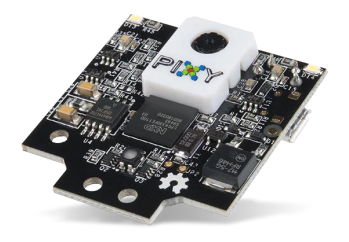
\includegraphics[width=0.5\textwidth]{pictures/chapter1/chapter1_pic15_camera.png}
                \caption{Camera SEN-14678 Pixy2 CMUcam5}
                \label{chap1_pic15}
            \end{figure}
        \subsubsection{Cảm biến hồng ngoại}
            \hspace*{0.6cm}Dựa trên nguyên lý phản xạ ánh sáng hồng ngoại (IR), để phân biệt giữa các vùng sáng - tối
            trên bề mặt di chuyển. Khi ánh sáng hồng ngoại được phát ra từ cảm biến và chiếu xuống mặt phẳng, cách mà bề mặt phản ứng lại với ánh sáng sẽ quyết định tín hiệu đầu ra.
            \begin{figure}[H]
                \centering
                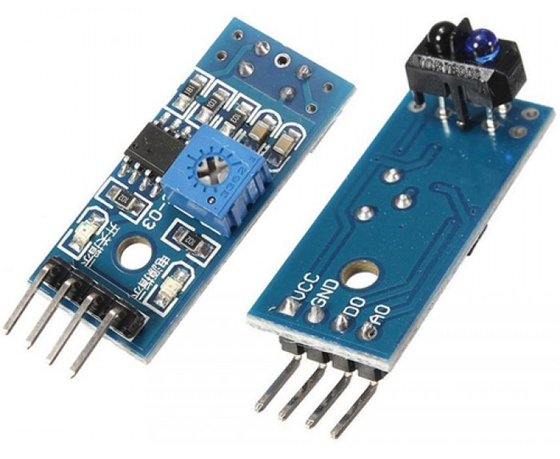
\includegraphics[width=0.4\textwidth]{pictures/chapter1/chapter1_pic17_IR.png}
                \caption{Cảm biến lò line hồng ngoại}
                \label{chap1_pic17}
            \end{figure}
            \textbf{1.4.1.2. Cảm biến quang trở}\\
            \hspace*{0.6cm}Quang điện trở, hay còn gọi tắt là RDL, là loại cảm biến ánh sáng đơn giản, hoạt động
                dựa vào hiện tượng quang điện trong. \newline
            \hspace*{0.6cm} Khi có ánh sáng chiếu vào chất bán dẫn, làm xuất hiện các điện tử tự do, làm sự
                dẫn điện tăng lên, làm giảm điện trở của chất bán dẫn (nếu có nối vào mạch điện thì
                mạch sẽ nối tắt, ngắn mạch). Khi không có ánh sáng chiếu vào, nội trở của chất bán dẫn
                tăng dần đến vô cùng (nếu có nối vào mạch điện thì sẽ hở mạch).
            \begin{figure}[H]
                \centering
                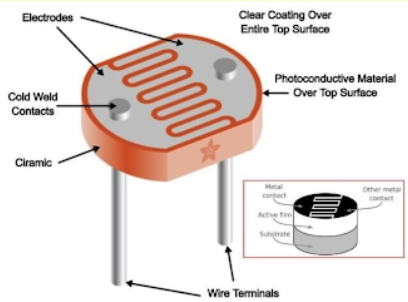
\includegraphics[width=0.4\textwidth]{pictures/chapter1/chapter1_pic16a_photoresistor.png}
                \caption{Cảm biến quang trở}
                \label{chap1_pic16}
            \end{figure}     

        \subsection{Cảm biến màu sắc}
            \hspace*{0.6cm}Để giải quyết nhiệm vụ nhận diện màu sắc, có thể sử dụng những cảm biến sau:
            \subsubsection{Cảm biến màu sắc}
                \hspace*{0.6cm} Cảm biến màu sắc hoạt động bằng cách chiếu ánh sáng (thường là từ đèn LED trắng hoặc RGB tích hợp trong cảm biến) lên bề mặt vật thể, 
                sau đó thu ánh sáng phản xạ lại. Ánh sáng này được tách thành các thành phần màu đỏ, xanh lá và xanh dương (RGB) thông 
                qua các bộ lọc hoặc photodiode. Cường độ từng màu được chuyển thành tín hiệu điện, từ đó bộ xử lý sẽ tính toán và xác định màu sắc của vật thể.
                \begin{figure}[H]
                    \centering
                    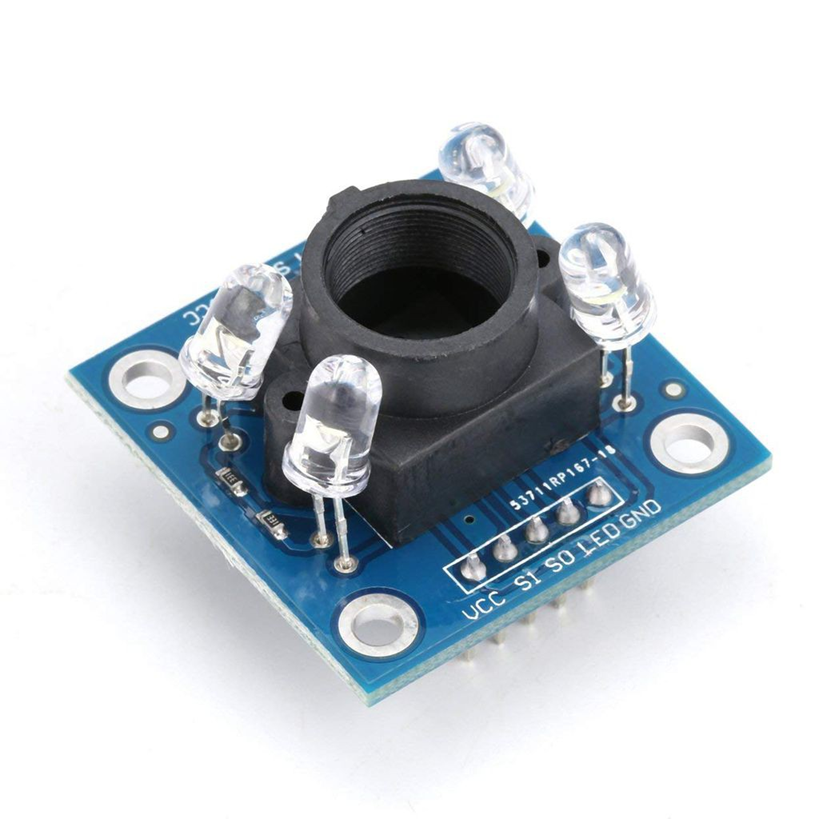
\includegraphics[width=0.4\textwidth]{pictures/chapter1/chapter1_pic18_color_sensor.png}
                    \caption{Cảm biến màu sắc}
                    \label{chap1_pic18}
                \end{figure}    
            \subsubsection{Camera}
                \hspace*{0.6cm}Dùng camera để chụp bề mặt vật thể, dùng xử lý ảnh để trích xuất thông tin màu.

    \section{Cấu trúc điều khiển}
        \subsection{Cấu trúc điều khiển phân cấp}
        \hspace*{0.6cm}Một MCU đóng vai trò như Master chỉ để tính toán cho chương trình điều
        khiển chính. Các Slave còn lại sử dụng các MCU khác để thực hiện các tác vụ riêng biệt
        như xử lý tín hiệu từ các cảm biến, tìm vị trí line, điều khiển driver, động cơ \dots
        %image
        \begin{figure}[H]
            \centering
            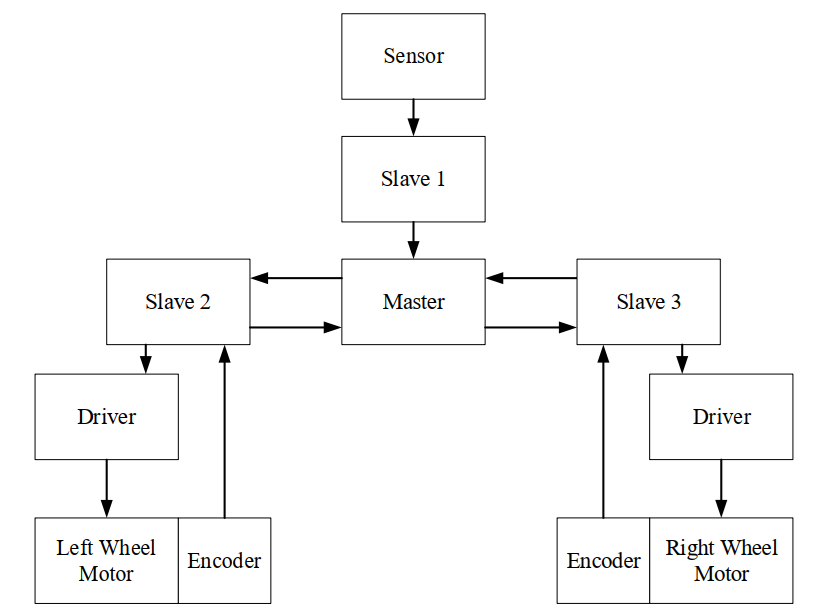
\includegraphics[width=0.8\textwidth]{pictures/chapter1/chapter1_pic19_phancap.png}
            \caption{Sơ đồ nguyên lý cấu trúc điều khiển phân cấp}
            \label{chap1_pic19}
        \end{figure}
        \begin{itemize}
            \item Ưu điểm: 
            \begin{itemize}[label=\textendash]
                \item Có tính linh hoạt cao trong việc quản lý, mở rộng và sửa chữa.
                \item Dễ dàng tìm kiếm và sửa chữa khi gặp lỗi.
                \item Có khả năng xử lý nhiều tác vụ cùng một lúc, giúp giảm thiểu thời gian xử lý cho mỗi vi điều khiển.
            \end{itemize}
            \item Nhược điểm: 
            \begin{itemize}[label=\textendash]
                \item Tốn thêm chi phí và không gian bố trí vi điều khiển.
                \item Tốn nhiều tài nguyên, phải quan tâm đến vấn đề giao tiếp giữa các MCU.
            \end{itemize}
        \end{itemize}
        \subsection{Cấu trúc điều khiển tập trung}
        \hspace*{0.6cm}Một MCU duy nhất đồng thời nhận và xử lý tín hiệu từ cảm biến, các encoder,
        thực hiện chương trình chính, tính toán và truyền giá trị điều khiển cho các động cơ.
        %image
        \begin{figure}[H]
            \centering
            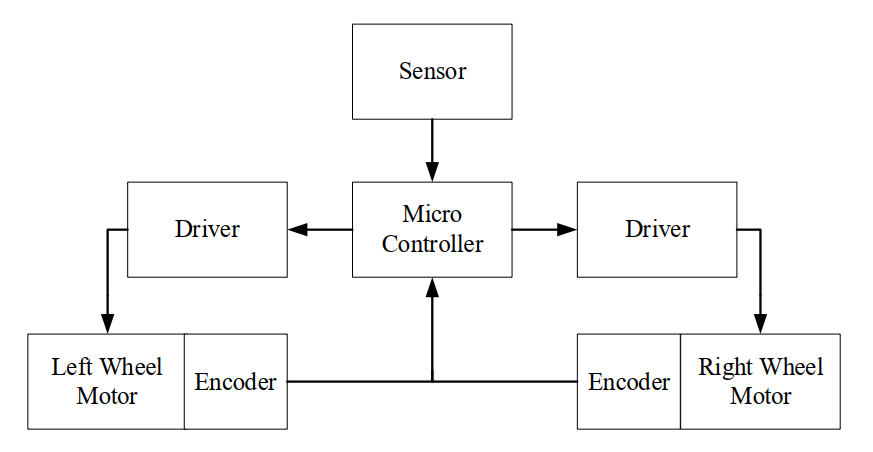
\includegraphics[width=0.8\textwidth]{pictures/chapter1/chapter1_pic20_taptrung.png}
            \caption{Sơ đồ nguyên lý cấu trúc điều khiển tập trung}
            \label{chap1_pic20}
        \end{figure}
        \begin{itemize}
            \item Ưu điểm: 
            \begin{itemize}[label=\textendash]
                \item Tiết kiệm được chi phí và không gian bố trí do chỉ sử dụng 1 MCU.
                \item Giảm khối lượng hệ thống.
                \item Không cần thực hiện giao tiếp giữa các vi điều khiển.
            \end{itemize}
            \item Nhược điểm: 
            \begin{itemize}[label=\textendash]
                \item Vi điều khiển không đủ chân I/O, analog, digital cần thiết.
                \item Đòi hỏi MCU có cấu hình mạnh, tốc độ xử lý cần thiết.
                \item Không có sự chuyên biệt hóa nên khó khăn trong việc tìm kiếm lỗi và sửa lỗi khi
                phát sinh lỗi chương trình.
            \end{itemize}
        \end{itemize}



    \section{Bộ điều khiển}
    \subsection{Bộ điều khiển PID}
    \hspace*{0.6cm}Bộ điều khiển PID là một bộ điều khiển dựa trên sai lệch giữa giá trị phản hồi
    thông qua cảm biến và giá trị mong muốn từ đó điều khiển được cơ cấu tác động thông
    qua các tham số P, I, D để đưa giá trị đầu ra gần với giá trị mong muốn nhất và ổn định
    nhất, với mỗi hệ thống khác nhau ta sẽ có các tham số của bộ điều khiển PID là khác
    nhau. Sai số giữa tâm xe và đường line sẽ được đưa vào bộ điều khiển PID xử lý, sau đó
    xuất ra lệnh điều khiển vận tốc ở hai động cơ trái và phải. Bộ điều khiển PID gồm 3
    phần chính là điều khiển P, I và D, đặc trưng bởi 3 hệ số $K_P, K_I, K_D$. Ngoài bộ PID đầy đủ, tùy theo mong muốn thiết kế có thể sử dụng bộ PI hoặc bộ PD.
    \begin{equation*}
        u(t) = K_P e(t) + K_I \int_0^t e(t) dt + K_D \dfrac{de(t)}{dt}
    \end{equation*}
    \begin{itemize}
        \item Ưu điểm: 
        \begin{itemize}[label = \textendash]
            \item Bộ điều khiển đơn giản, phù hợp với những hệ thống đơn giản, ít bị nhiễu.
            \item Dễ thiết kế và và điều chỉnh các hệ số PID.
        \end{itemize}
        \item Nhược điểm:
        \begin{itemize}[label = \textendash]
            \item Hiệu quả kém khi hệ thống phi tuyến hoặc bị ảnh hưởng bởi nhiễu lớn.
            \item Cần thực nghiệm nhiều lần để tìm ra bộ hệ số tối ưu cho bộ điều khiển.
        \end{itemize}
    \end{itemize}
    \subsection{Bộ điều khiển fuzzy}
    \hspace*{0.6cm}Bộ điều khiển Fuzzy là một bộ điều khiển dựa trên việc sử dụng quy tắc fuzzy IFTHEN, giúp mô tả vấn đề một đơn giản và nhanh chóng. Bộ điều khiển fuzzy phủ hợp
    cho cả hệ thống tuyến tính lẫn phi tuyến nhờ vào kiến thức và kinh nghiệm của người
    thiết kế. Đối với hệ thống xe AGV, bộ điều khiển fuzzy cho phép điều khiển xe trong
    nhiều điều kiện hoàn cảnh khác nhau khắc phục được những hạn chế của lýthuyết điều
    khiển kinh điển.
    \newline
    \hspace*{0.6cm}Cấu trúc của bộ điều khiển fuzzy:
    \begin{itemize}[label=\textendash]
        \item Khâu mờ hóa: Chuyển các điều kiện có giá trị cụ thể thành những khoảng phù
        hợp thao tác kinh nghiệm và sự hiểu biết hệ thống của người lập trình ứng kết quả mong
        muốn tương ứng.
        \item Thực hiện luật hợp thành: hình thành luật mờ theo dạng IF \dots THEN.
        \item Khâu giải mờ: từ luật hợp thành tính toán ra giá trị kết quả trong những trường
        hợp cụ thể. Sử dụng phương pháp cực đại, phương pháp trọng tâm \dots.
        \begin{figure}[H]
            \centering
            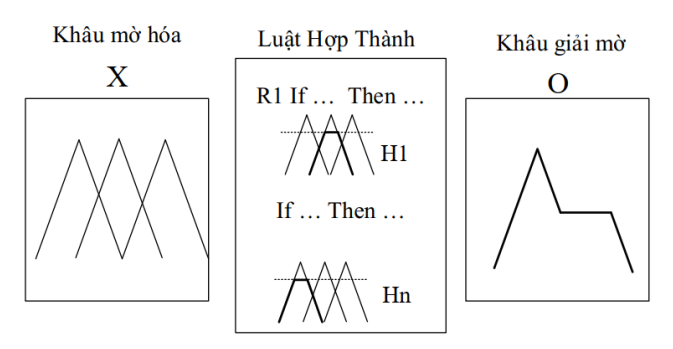
\includegraphics[width=0.6\textwidth]{pictures/chapter1/chapter1_pic21_fuzzy.png}
            \caption{Bộ điều khiển fuzzy}
            \label{chap1_pic21}
        \end{figure}          
    \end{itemize}

    \begin{itemize}
        \item Ưu điểm: 
        \begin{itemize}
            \item Bộ điều khiển phù hợp cho những hệ thống phi tuyến, thiết kế dựa trên kinh nghiệm của người thiết kế về hệ thống.
            \item Chịu ảnh hưởng ít hơn bởi nhiễu của môi trường.
        \end{itemize}
        \item Nhược điểm:
        \begin{itemize}
            \item Thiết kế phức tạp hơn, cần xác định luật mờ, hàm phụ thuộc.
            \item Không có tham số rõ ràng như bộ điều khiển PID, cần hiểu biết rõ ràng về hệ thống.
        \end{itemize}
    \end{itemize} 
    \subsection{Điều khiển dùng hàm Lyapunov}
    \hspace*{0.6cm}Phương pháp điều khiển dùng hàm Lyapunov dùng cách tiếp cận thiết kế luật điều khiển sao cho đảm bảo tính ổn định của hệ thống dựa trên định lý ổn định Lyapunov. Ý tưởng là
    \begin{itemize}[label=\textendash]
        \item Chọn hàm Lyapunov $V(x)$ phù hợp cho hệ thống.
        \item Thiết kế luật điều khiển $ u(t) $ sao cho hệ thống ổn định dựa trên định lý ổn định Lyapunov. 
    \end{itemize}
    \hspace*{0.6cm}Trong đó hàm Lyapunov được dùng như 1 công cụ để chứng minh tính ổn định của 1 hệ thống động lực học (hệ thống hội tụ về trạng thái cân bằng hoặc một trạng thái mong muốn) mà không cần giải phương trình vi phân của hệ thống.
    \begin{itemize}
        \item Ưu điểm: 
        \begin{itemize}[label=\textendash]
            \item Xử lý được với các hệ phi tuyến.
            \item Đảm bảo tính ổn định của hệ thống nhờ phương pháp tiếp cận chặt chẽ về mặt toán học.
            \item Linh hoạt trong thiết kế bộ điều khiển thông qua việc thay đổi lựa chọn các hàm Lyapunov khác nhau.
            \item Không cần giải phương vi phân của hệ thống.
        \end{itemize}
        \item Nhược điểm:
        \begin{itemize}[label=\textendash]
            \item Việc lựa chọn hàm Lyapunov tối ưu đòi hỏi hiểu biết rõ ràng về hệ thống.
            \item Không tối ưu về hiệu suất vì phương pháp tập trung vào cải thiện tính ổn định của hệ thống thay vì đảm bảo tối ưu các yếu tố khác.
            \item Với những hệ thống phức tạp, việc tính toán có thể trở nên khó khăn.
            \item Trong thực tế, xe dò line thường sử dụng các loại vi điều khiển cơ bản. Việc triển khai luật điều khiển phức tạp từ phương pháp Lyapunov đòi hỏi tài nguyên tính toán lớn hơn so với các phương pháp đơn giản như PID.
        \end{itemize}
    \end{itemize}        


    \section{Đầu bài cụ thể}
        \hspace*{0.6cm}Các ràng buộc về điều kiện của đầu bài cụ thể được đưa ra như sau:
        \begin{itemize}
            \item Bề mặt sa bàn không có nếp gấp, độ nhấp nhô tối đa $\pm 10$ (mm).
            \item Độ rọi của phòng: $I = 300 - 500$ (lux).
            \item Không chịu tác động lực ngoài phạm vi đề bài.
            \item Sai số bám đường dẫn là $\pm 3$ (mm).
            \item Sai số vị trí dừng cuối đường dẫn là $\pm 5$ (mm).
            \item Khối lượng có thể tải là $m = 1.5$ (kg).
            \item Vật tải phải được đặt ở vị trí đã được bố trí trên xe. Màu vật tải được quy định là màu đỏ tươi và màu xanh lam.
        \end{itemize}
        \hspace*{0.6cm}Từ các ràng buộc trên và yêu cầu của đề bài, nhóm sẽ tiến hành thiết kế robot bám line phân loại hàng hóa theo màu sắc với cá thông số sau:
        \begin{table}[H]
            \centering
            \caption{Bảng thông số đầu bài}
            \begin{tabular}{|l|c|}
            \hline
            \centering \textbf{Thông số} & \textbf{Giá trị} \\
            \hline
            Vận tốc xe trung bình & $v_{max} = 0.5$ (m/s) \\
            \hline
            Bán kính cong nhỏ nhất & $\rho_{min} = 500$ (mm) \\
            \hline
            Bề rộng đường dẫn & 26 (mm) \\
            \hline
            Sai số bám đường dẫn & $\pm 3$ (mm) \\
            \hline
            Sai số vị trí dừng cuối đường dẫn & $\pm 5$ (mm) \\
            \hline
            Sai số vị trí xuất phát & $\pm 5$ (mm) \\
            \hline
            Khối lượng có thể tải & $m = 1$ (kg) \\
            \hline
            \end{tabular}
        \end{table}





    